\documentclass[a4paper,oneside,DIV=12,12pt]{scrartcl}

\usepackage{graphicx}

\usepackage{fontspec}
\setmainfont{STIX Two Text}
\setsansfont{Roboto}

\usepackage{microtype}

\usepackage{polyglossia}
\setmainlanguage{ukrainian}

%%% Math typesetting
\usepackage{amsmath}
\usepackage{unicode-math}
\setmathfont{STIX Two Math}
\usepackage[retainorgcmds]{IEEEtrantools}
%%%

%%% Table typesetting
\usepackage{booktabs}
\usepackage{longtable}
%%%

%%% Captions
\usepackage{caption}
\usepackage{subcaption}
%%%

%%% SI units typesetting
\usepackage{siunitx}
\sisetup{output-decimal-marker = {,},
exponent-product = {\cdot}}
%%%

%%% Tikz
\usepackage{tikz}
\usetikzlibrary{arrows.meta}
\usetikzlibrary{quotes}

\usepackage{tikzscale}
%%%

\newcommand\schel[1]{\textit{#1}}

\begin{document}
	\begin{titlepage}
		\begin{center}
			Міністерство освіти і науки України\\
			Національний авіаційний університет\\
			Навчально-науковий інститут комп'ютерних інформаційних технологій\\
			Кафедра комп'ютеризованих систем управління
			
			\vspace{\fill}
				Лабораторна робота №4\\
				з дисципліни «Теорія електричних та магнітних кіл»\\
				на тему: «Розрахунок складного електричного~кола синусоїдного~струму з~експериментальною~перевіркою»\\
				% Варіант №
				
			\vspace{\fill}
			
			\begin{flushright}
				Виконав:\\
				студент ННІКІТ СП-225\\
				Клокун Владислав\\
				Перевірив:\\
				Молчанов О.~В.
			\end{flushright}
			Київ 2017
		\end{center}
	\end{titlepage}
	
	\section{Мета роботи}
		\begin{enumerate}
			\item Набути необхідні навички практичного розрахунку складного електричного кола синусоїдного струму, використовуючи методи аналізу кіл.
			\item Перевірити правильність розрахунку кола, використовуючи рівняння балансу потужностей.
			\item Навчитися будувати векторну діаграму струмів та топографічну діаграму напруг контуру.
		\end{enumerate}
		
	% \section{Короткі теоретичні відомості}
		% Для розрахунку кіл змінного струму застосовують такі ж методи, що і для аналізу кіл постійного струму, а саме метод рівнянь Кірхгофа, методи контурних струмів, вузлових потенціалів, еквівалентних перетворень і т.п. Однак, ці методи аналізу можна застосовувати тільки в сукупності з теорією комплексних змінних.
		
		% Відомо, що синусоїдні функції часу
		% \[
			% i(t) = I_m \sin(\omega t + \varphi_i), \quad
			% u(t) = U_m \sin(\omega t + \varphi_i),
		% \]
		% якими описуються миттєві значення змінних струмів і напруг, можна представити у вигляді комплексних чисел:
		% \[
			% I_m = I_m e^{j \varphi_i}, \quad
			% U_m = U_m e^{j \varphi_i},
		% \]
		% у яких.
	
	\section{Порядок виконання роботи}
		Для виконання даної лабораторної роботи можна використовувати лабораторний стенд №8 або скористатися магазинами резисторів, індуктивностей та ємностей. Але в будь-якому випадку необхідно зібрати вимірювальну частину схеми, зображеної на рисунку~\ref{fig:schematic-01} і по черзі провести необхідні вимірювання, підключаючи до виходу схеми елементи, вказані в таблиці~\ref{tab:measurement-01}.
		
		\begin{figure}[!htbp]
		\centering
			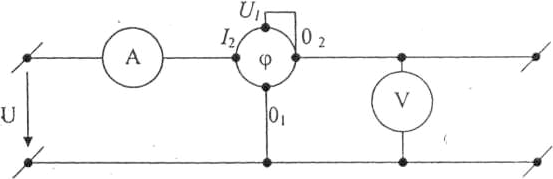
\includegraphics[height = 8\baselineskip]{schematic-01.png}
		\caption{Схема №1}
		\label{fig:schematic-01}
		\end{figure}
		
		\begin{longtable}[c]{
			l
			S[table-format = 2.1]
			S[table-format = 3e-1]
			S[table-format = +2, retain-explicit-plus]
		}
			\toprule
				Параметри & {$U, \si{\volt}$} & {$I, \si{\ampere}$} & {$\varphi, \si{\degree}$}\\
			\midrule
			\endhead
			\bottomrule
			\caption{Дані №1}
			\endfoot
			\label{tab:measurement-01}
			
				\schel{R1} & 20   & 327e-3 & 0 \\
				\schel{R2} & 20   & 122e-3 & 0 \\
				\schel{L}  & 20.8 & 133e-3 & +80 \\
				\schel{R4} & 20   & 82e-3  & 0 \\
				\schel{C}  & 21.8 & 129e-3 & -90 \\

		\end{longtable}
		
		Використовуючи дані таблиці~\ref{tab:measurement-01}, розрахувати значення активних опорів резисторів \schel{R1}, \schel{R2}, \schel{$R_{\text{К}}$}, \schel{R4}, \schel{$R_C$} і значення реактивних опорів індуктивності та ємності \schel{$X_{\text{К}}$}, \schel{$X_C$}. З'ясувати у викладача кількість джерел ЕРС, позначення та значення їх напруги у схемі, при яких необхідно розрахувати задане коло, і методи аналізу цього кола. Всі отримані дані занести у таблицю~\ref{}.
		
		\begin{table}[!htbp]
		\centering
			\begin{tabular}{
				S[table-format = 2]
				S[table-format = 1]
				S[table-format = 1]
				S[table-format = 2.1]
				S[table-format = 3.1]
				S[table-format = 2]
				S[table-format = 3.1]
				S[table-format = 3]
				S[table-format = 1]
				S[table-format = 3]
			}
				\toprule
					{$E_1, \si{\volt}$} &
					{$E_2, \si{\volt}$} &
					{$E_1, \si{\volt}$} &
					{$\schel{R1}, \si{\ohm}$} &
					{$\schel{R2}, \si{\ohm}$} &
					{$R_{\text{K}}, \si{\ohm}$} &
					{$X_{\text{К}}, \si{\ohm}$} &
					{$\schel{R4}, \si{\ohm}$} &
					{$R_C, \si{\ohm}$} &
					{$X_C, \si{\ohm}$}\\
				\midrule
					 30 & 0 & 0 & 61.1 & 163.9 & 26 & 154.2 & 243 & 0 & 169\\
				\bottomrule
			\end{tabular}
		\caption{Дані №2}
		\label{}
		\end{table}
		
		Розрахувати електричне коло на рисунку~\ref{fig:schematic-02} відповідно до завдання, використовуючи символічний метод розрахунку. Тобто необхідно визначити діючі значення струмів схеми заданими методами та діючі значення напруг на елементах кола. Перевірити правильність розрахунку кола за рівняннями балансу потужностей. Дані розрахунку занести в таблицю~\ref{tab:measurements-03}.
		
		\begin{figure}[!htbp]
		\centering
			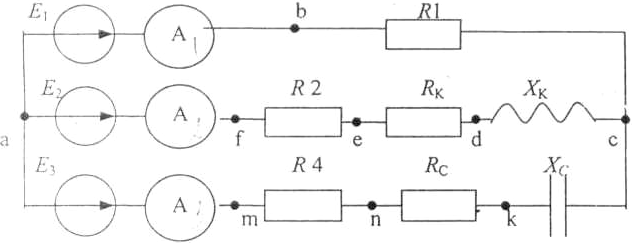
\includegraphics[height = 8\baselineskip]{schematic-02.png}
		\caption{Схема №2}
		\label{fig:schematic-02}
		\end{figure}
		
		Зібрати електричну схему на рисунку~\ref{fig:schematic-02}, включивши в неї необхідні вимірювальні прилади. Виконати вимірювання струмів і напруг. Результати експерименту занести в таблицю~\ref{tab:measurements-03}.
		
		Використовуючи результати попередніх пунктів, обчислити похибку отриманих результатів. Результати обчислень занести в таблицю~\ref{tab:measurements-03}.
		
		Побудувати векторну діаграму струмів і топографічну діаграму напруг.
		
		\begin{longtable}[c]{
				l
				S[table-format = 2.1]
				S[table-format = 3e-1]
				S[table-format = 3e-1]
				S[table-format = 3e-1]
				S[table-format = 2.1]
				S[table-format = 2.1]
				S[table-format = 2.1]
				S[table-format = 2.1]
				S[table-format = 2.1]
			}
				\toprule
					Метод &
					{$U$} &
					{$I_1$} &
					{$I_2$} &
					{$I_3$} &
					{$U_{bc}$} &
					{$U_{ce}$} &
					{$U_{ef}$} &
					{$U_{cn}$} &
					{$U_{nm}$} \\
				\midrule
				\endhead
				\bottomrule
				\caption{Експериментальні та теоретичні дані}
				\endfoot
				\label{tab:measurements-03}
				
					МКС     & 25       & 124e-3   & 78e-3    & 54e-3    & 7.6      & 12.2     & 13       & 9.1      & 13.2 \\
					МВП     & 17.7     & 180e-3   & 90e-3    & 30e-3    & 17       & 6.2      & 6.5      & 5.1      & 7.3\\
					Дослід  & 30       & 132e-3   & 85e-3    & 55e-3    & 8.6      & 12.2     & 14.5     & 12.1     & 16.9\\
					Похибка & {$16\%$} & {$6\%$} & {$8\%$} & {$2\%$} & {$11\%$} & {$0\%$} & {$8\%$} & {$24\%$} & {$21\%$} \\
		\end{longtable}
		
	\section{Розрахунки}
		\subsection{Метод контурних струмів}
			У схемі два контури. Обравши напрямки їх обходу так, щоб вони співпадали, складаємо систему рівнянь для методу контурних струмів:
			\[
				\left\{
					\begin{IEEEeqnarraybox}[
						\IEEEeqnarraystrutmode
						\IEEEeqnarraystrutsizeadd{2pt}{2pt}
					][c]{l}
						I_{11}  \left( Z_1 + Z_2 + Z_K \right) + I_{22}  \left( Z_2 + Z_K \right) = E_1,\\
						I_{11}  \left( Z_2 + Z_K \right)       + I_{22}  \left( Z_2 + Z_U + Z_4 + Z_C \right) = 0.
					\end{IEEEeqnarraybox}
				\right.
			\]
			
			Підставимо дослідні значення: $Z_1 = R_1$, $Z_2 = R_2$, $Z_3 = R_4$. Обчислимо значення опорів, що не вказані:
			\begin{IEEEeqnarray*}{rCcCl}
				Z_U &=& \sqrt{R_K^2 + X_K^2} &=& \num{156.37},\\
				Z_C &=& \sqrt{R_C^2 + X_C^2} &=& \num{169}.
			\end{IEEEeqnarray*}
			
			Отримали систему лінійних алгебраїчних рівнянь:
			\begin{IEEEeqnarray*}{c}
				\left\{
					\begin{IEEEeqnarraybox}[
						\IEEEeqnarraystrutmode
						\IEEEeqnarraystrutsizeadd{2pt}
						{2pt}
					][c]{rrCrrCl}
						381 & I_{11} &+& 320 & I_{22} &=& 30,\\
						320 & I_{11} &+& 732 & I_{22} &=& 0.
					\end{IEEEeqnarraybox}
				\right.
				\implies
				\left|
					\begin{array}{rr|r}
						381 & 320 & 30\\
						320 & 732 & 0\\
					\end{array}
				\right|
			\end{IEEEeqnarray*}
			
			Звідси $\Delta = \num{1766492}$, $\Delta_1 = 21960$, $\Delta_2 = -9600$. Знаходимо перший контурний струм~$I_{11} = \Delta_1 / \Delta = \SI{0.1244}{\ampere}$; другий контурний струм~$I_{22} = \Delta_2 / \Delta = \SI{-0.0543}{\ampere}$. Знаходимо реальні струми: $I_1 = \SI{0.1244}{\ampere}$, $I_2 = I_K = \SI{0.0787}{\ampere}$, $I_3 = I_C = \SI{-0.0543}{\ampere}$.
			
		\subsection{Метод вузлових потенціалів}
			Оскільки у схемі два вузли, з яких вузол~$\varphi_1$ заземлюється для проведення обчислень, рівняння, складене за методом вузлових потенціалів, має вигляд:
			\[
				U_1 \left( V_1 + V_2 + V_K + V_U + V_E \right) = E_1 V_1.
			\]
			
			Виражаємо струми:
			\[
				I_1 = \frac{-\varphi_1 + E_1}{Z_1}, \quad
				I_2 = I+K = \frac{\varphi_1}{\left( Z_2 + Z_K\right)}, \quad
				I_3 = I_C = \frac{-\varphi_1}{\left( Z_4 + Z_C \right)}.
			\]
			
			Виражаємо потенціали:
			\[
				V_1 = \frac{1}{R_1}, \quad
				V_2 = \frac{1}{R_2}, \quad
				V_3 = \frac{1}{R_4}, \quad
				V_K = \frac{1}{\sqrt{R_K^2 + X_K^2}}, \quad
				V_C = \frac{1}{\sqrt{R_C^2 + X_C^2}}.
			\]
			
			Звідси отримали: $\num{0.3888} \varphi_1 = \num{0.49}$, тобто $\varphi_1 = \SI{12.628}{\volt}$. Знайдені значення струмів: $I_1 = \SI{0.28}{\ampere}$, $I_2 = \SI{0.04}{\ampere}$, $I_3 = \SI{-0.03}{\ampere}$.
			
		\section{Діаграми}
			Під час виконання лабораторної роботи була побудована топографічна діаграма напруг~(рис.~\ref{fig:topological-diagram}).
			
			\begin{figure}[!htbp]
			\centering
				\includegraphics[height = 12\baselineskip]{assets/topological-diagram.tikz}
			\caption{Топографічна діаграма напруг}
			\label{fig:topological-diagram}
			\end{figure}
		
	\section{Висновки}
		Виконуючи дану лабораторну роботу, ми набули необхідні навички практичного розрахунку складного електричного кола синусоїдного струму, використовуючи методи аналізу кіл; перевірили правильність розрахунку кола, використовуючи рівняння балансу потужностей, а також навчились будувати векторну діаграму струмів та топографічну діаграму напруг контуру.
		
\end{document}